% (find-LATEX "2021-2-C3-funcoes-quadraticas.tex")
% (defun c () (interactive) (find-LATEXsh "lualatex -record 2021-2-C3-funcoes-quadraticas.tex" :end))
% (defun C () (interactive) (find-LATEXsh "lualatex 2021-2-C3-funcoes-quadraticas.tex" "Success!!!"))
% (defun D () (interactive) (find-pdf-page      "~/LATEX/2021-2-C3-funcoes-quadraticas.pdf"))
% (defun d () (interactive) (find-pdftools-page "~/LATEX/2021-2-C3-funcoes-quadraticas.pdf"))
% (defun e () (interactive) (find-LATEX "2021-2-C3-funcoes-quadraticas.tex"))
% (defun o () (interactive) (find-LATEX "2021-1-C3-funcoes-quadraticas.tex"))
% (defun u () (interactive) (find-latex-upload-links "2021-2-C3-funcoes-quadraticas"))
% (defun v () (interactive) (find-2a '(e) '(d)))
% (defun d0 () (interactive) (find-ebuffer "2021-2-C3-funcoes-quadraticas.pdf"))
% (defun cv () (interactive) (C) (ee-kill-this-buffer) (v) (g))
%          (code-eec-LATEX "2021-2-C3-funcoes-quadraticas")
% (find-pdf-page   "~/LATEX/2021-2-C3-funcoes-quadraticas.pdf")
% (find-sh0 "cp -v  ~/LATEX/2021-2-C3-funcoes-quadraticas.pdf /tmp/")
% (find-sh0 "cp -v  ~/LATEX/2021-2-C3-funcoes-quadraticas.pdf /tmp/pen/")
%     (find-xournalpp "/tmp/2021-2-C3-funcoes-quadraticas.pdf")
%   file:///home/edrx/LATEX/2021-2-C3-funcoes-quadraticas.pdf
%               file:///tmp/2021-2-C3-funcoes-quadraticas.pdf
%           file:///tmp/pen/2021-2-C3-funcoes-quadraticas.pdf
% http://angg.twu.net/LATEX/2021-2-C3-funcoes-quadraticas.pdf
% (find-LATEX "2019.mk")
% (find-CN-aula-links "2021-2-C3-funcoes-quadraticas" "3" "c3m212q" "c3q")

% «.defs»			(to "defs")
% «.title»			(to "title")
% «.point-of-view»		(to "point-of-view")
% «.figuras-3D»			(to "figuras-3D")
% «.exercicio-1»		(to "exercicio-1")
% «.exercicio-2»		(to "exercicio-2")
% «.exercicio-3»		(to "exercicio-3")
% «.exercicio-4»		(to "exercicio-4")
% «.zt-e-ztt-intro»		(to "zt-e-ztt-intro")
% «.exercicio-5»		(to "exercicio-5")
% «.ztt-matematicos»		(to "ztt-matematicos")
% «.ztt-matematicos-2»		(to "ztt-matematicos-2")
% «.ztt-matematicos-3»		(to "ztt-matematicos-3")
% «.gardner-1»			(to "gardner-1")
% «.gardner-2»			(to "gardner-2")
% «.thompson-1»			(to "thompson-1")
% «.thompson-2»			(to "thompson-2")
% «.thompson-3»			(to "thompson-3")
% «.thompson-inversa-1»		(to "thompson-inversa-1")
% «.thompson-inversa-2»		(to "thompson-inversa-2")
% «.g-m-diff»			(to "g-m-diff")
% «.useful-dodge»		(to "useful-dodge")
% «.exercicio-6»		(to "exercicio-6")
% «.derivada-direcional»	(to "derivada-direcional")
%
% «.djvuize»			(to "djvuize")




% <videos>
% Video (not yet):
% (find-ssr-links     "c3m212q" "2021-2-C3-funcoes-quadraticas")
% (code-eevvideo      "c3m212q" "2021-2-C3-funcoes-quadraticas")
% (code-eevlinksvideo "c3m212q" "2021-2-C3-funcoes-quadraticas")
% (find-c3m212qvideo "0:00")

\documentclass[oneside,12pt]{article}
\usepackage[colorlinks,citecolor=DarkRed,urlcolor=DarkRed]{hyperref} % (find-es "tex" "hyperref")
\usepackage{amsmath}
\usepackage{amsfonts}
\usepackage{amssymb}
\usepackage{pict2e}
\usepackage[x11names,svgnames]{xcolor} % (find-es "tex" "xcolor")
\usepackage{colorweb}                  % (find-es "tex" "colorweb")
%\usepackage{tikz}
%
% (find-dn6 "preamble6.lua" "preamble0")
%\usepackage{proof}   % For derivation trees ("%:" lines)
%\input diagxy        % For 2D diagrams ("%D" lines)
%\xyoption{curve}     % For the ".curve=" feature in 2D diagrams
%
\usepackage{edrx21}               % (find-LATEX "edrx21.sty")
\input edrxaccents.tex            % (find-LATEX "edrxaccents.tex")
\input edrx21chars.tex            % (find-LATEX "edrx21chars.tex")
\input edrxheadfoot.tex           % (find-LATEX "edrxheadfoot.tex")
\input edrxgac2.tex               % (find-LATEX "edrxgac2.tex")
%
%\usepackage[backend=biber,
%   style=alphabetic]{biblatex}            % (find-es "tex" "biber")
%\addbibresource{catsem-slides.bib}        % (find-LATEX "catsem-slides.bib")
%
% (find-es "tex" "geometry")
\usepackage[a6paper, landscape,
            top=1.5cm, bottom=.25cm, left=1cm, right=1cm, includefoot
           ]{geometry}
%
\begin{document}

\catcode`\^^J=10
\directlua{dofile "dednat6load.lua"}  % (find-LATEX "dednat6load.lua")

%L dofile "edrxtikz.lua"  -- (find-LATEX "edrxtikz.lua")
%L dofile "edrxpict.lua"  -- (find-LATEX "edrxpict.lua")
%L dofile "2021-1-C3-3D.lua" -- (find-LATEX "2021-1-C3-3D.lua")
%L
%L V3.__index.tostring = function (v) return v:v2string() end
\pu

% «defs»  (to ".defs")
% (find-LATEX "edrx21defs.tex" "colors")
% (find-LATEX "edrx21.sty")

\def\u#1{\par{\footnotesize \url{#1}}}

\def\thompsonpage#1{{\scriptsize
\url{https://www.gutenberg.org/files/33283/33283-pdf.pdf\#page=#1}
}}

\def\pictgray#1{{\color{GrayPale}\linethickness{0.3pt}#1}}

\def\drafturl{http://angg.twu.net/LATEX/2021-2-C3.pdf}
\def\drafturl{http://angg.twu.net/2021.2-C3.html}
\def\draftfooter{\tiny \href{\drafturl}{\jobname{}} \ColorBrown{\shorttoday{} \hours}}



%  _____ _ _   _                               
% |_   _(_) |_| | ___   _ __   __ _  __ _  ___ 
%   | | | | __| |/ _ \ | '_ \ / _` |/ _` |/ _ \
%   | | | | |_| |  __/ | |_) | (_| | (_| |  __/
%   |_| |_|\__|_|\___| | .__/ \__,_|\__, |\___|
%                      |_|          |___/      
%
% «title»  (to ".title")
% (c3m212qp 1 "title")
% (c3m212qa   "title")

\thispagestyle{empty}

\begin{center}

\vspace*{1.2cm}

{\bf \Large Cálculo 3 - 2021.2}

\bsk

Aula 17: algumas funções quadráticas

\bsk

Eduardo Ochs - RCN/PURO/UFF

\url{http://angg.twu.net/2021.2-C3.html}

\end{center}

\newpage

{\bf Introdução}

Nós começamos a ver como pegar uma superfície e um ponto

dela e aí obter um plano tangente a essa superfície nesse ponto,

e começamos a ver qual é a relação disso com derivadas parciais...

\msk

Um plano tangente é uma {\sl aproximação de 1ª ordem}.

Nestes exercícios vamos ver um pouco sobre aproximações

de 2ª ordem --- mas só o suficiente pra gente ter mais motivação

pra ``notação de físicos'' e pra gente aprender a visualizar o que

certas contas importantes querem dizer.


\msk

O que a gente vai ver aqui tem muito a ver com as superfícies

quádricas que costumam ser vistas rapinho no final do curso

de GA, mas vamos usar alguns truques pro nosso ponto base

não precisar ser o zero. Veja as figuras 3D daqui...

\msk

{\scriptsize

\url{https://en.wikipedia.org/wiki/Quadric}

}


\newpage

{\bf A equação da superfície}

Nós vamos usar esta equação pra nossa superfície:
%
$$\begin{array}{rcl}
  z &=& z(x,y) \\
    &=& z(x_1,y_1) \\
    &=& a + b·(x_1-x_0) + c·(y_1-y_0) \\
    &+& d·(x_1-x_0)^2 + e·(x_1-x_0)(y_1-y_0) \\
    &+& f·(y_1-y_0)^2 \\
    &=& a + bΔx + cΔy + dΔx^2 + eΔxΔy + fΔy^2 \\
  \end{array}
$$

Repare que vamos usar $x=x_1$ e $y=y_1$ pra podermos

usar as convenções $Δx=x_1-x_0$ e $Δy=y_1-y_0$ sem

precisamos definir nada extra.

\msk

Nas figuras dos próximos slides vamos sempre usar

$x_0=3$ e $y_0=2$.

\newpage

% «point-of-view»  (to ".point-of-view")
% (c3m211qp 4 "point-of-view")
% (c3m211qa    "point-of-view")

% (find-LATEX "2021-1-C3-3D.lua" "QuadraticFunction-tests")
%L
%L V3.__index.p1 = V{2, -0.5}
%L V3.__index.p2 = V{1,  1.5}
%L V3.__index.p3 = V{0,  2}
%L
%L V3.__index.p1 = V{2,   -0.5}
%L V3.__index.p2 = V{0.5, 1.7}
%L V3.__index.p3 = V{0,   0.5}
%L
%L setsrf = function (tbl)
%L     tbl.x0 = 3
%L     tbl.y0 = 2
%L     qf = QuadraticFunction(tbl)
%L     srf = Surface.new(qf, 3, 2)
%L   end
\pu
\def\setsrf#1{\directlua{setsrf({#1})}}

\def\QuadraticInPerspective#1{
   \myvcenter{
   \beginpicture(0,-3)(10,6)
     \pictgray{\expr{v3():xygrid(4,3)          }}
     \expr          {v3():axeswithticks(4,3,3) }
     \expr          {#1:diagonals(8, "c")      }
     \expr          {#1:square   (8, "0")      }
     \pictgray{\expr{#1:square   (2, "p")      }}
     \expr          {#1:square   (8, "c")      }
   \end{picture}}}

% ----------------------------------------

% «figuras-3D»  (to ".figuras-3D")
% (c3m211qp 4 "figuras-3D")
% (c3m211qa   "figuras-3D")

\unitlength=8pt

\def\QP#1#2{
  \begin{array}{c}
    \setsrf {#1}
    \QuadraticInPerspective{srf} \\
    #2
  \end{array}
  }

\pu

$$\begin{array}{c}
   \QP {a=2} {z = 2}
   \quad
   \QP {a=2, Dx=1} {z = 2+Δx}
   \quad
   \QP {a=2, Dxx=1} {z = 2+Δx^2}
  \\
  \\
   \QP {a=2} {z = 2}
   \quad
   \QP {a=2, Dy=1} {z = 2+Δy}
   \quad
   \QP {a=2, Dyy=1} {z = 2+Δy^2}
  \end{array}
$$


\newpage

$$\begin{array}{c}
   \QP {a=2, Dx=1, Dy=1} {z = 2 + (Δx + Δy)}
   \quad
   \QP {a=2, Dxx=1, Dyy=1, Dxy=2} {z = 2 + (Δx + Δy)^2}
  \\
  \\
   \QP {a=2, Dx=-1, Dy=1}          {z = 2 + (Δy - Δx)}
   \quad
   \QP {a=2, Dxx=1, Dyy=1, Dxy=-2} {z = 2 + (Δy - Δx)^2}
  \end{array}
$$


\newpage

% «exercicio-1»  (to ".exercicio-1")
% (c3m211qp 6 "exercicio-1")
% (c3m211qa   "exercicio-1")

{\bf Exercício 1.}

Faça o diagram de numerozinhos de cada uma das superfícies

abaixo. Considere que os pontos que nos interessam são só

os em que $x∈\{x_0-1, x_0, x_0+1\}$ e $y∈\{x_0-1, x_0, x_0+1\}$.

Veja o vídeo pra entender!

\msk

\begin{tabular}[t]{l}
a) $z = 2$ \\
b) $z = x$ \\
c) $z = Δx$ \\
d) $z = Δx^2$ \\
e) $z = Δx^2 + 2$ \\
\end{tabular}
\msk
\begin{tabular}[t]{l}
f) $z = y$ \\
g) $z = Δy$ \\
h) $z = Δy^2$ \\
i) $z = Δy^2 + 2$ \\
j) $z = Δx^2+Δy^2$ \\
k) $z = Δx^2+Δy^2 + 2$ \\
\end{tabular}
\msk
\begin{tabular}[t]{l}
l) $z = Δx+Δy$ \\
m) $z = (Δx+Δy)^2$ \\
n) $z = (Δx+Δy)^2 + 2$ \\
\end{tabular}

\newpage

% «exercicio-2»  (to ".exercicio-2")
% (c3m211qp 7 "exercicio-2")
% (c3m211qa   "exercicio-2")

{\bf Exercício 2.}

Relembre o que era o ``estudo do sinal de uma função''

que você deve ter visto em Cálculo 1, e faça um diagramas

indicando em que intervalos cada uma das funções abaixo

é positiva, negativa, ou zero.

(Veja o segundo vídeo!)

\msk

a) $x$

b) $x+1$

c) $x(x+1)$

d) $4-x$

e) $x(x+1)(4-x)$

\newpage

% «exercicio-3»  (to ".exercicio-3")
% (c3m211qp 8 "exercicio-3")
% (c3m211qa   "exercicio-3")

{\bf Exercício 3.}

Agora adapte essa idéia do diagrama do sinal para $\R^2$,

no quadrado com $x∈[x_0-1,x_0+1]$ e $y∈[y_0-1,y_0+1]$,

e faça o diagrama do sinal para cada uma das funções abaixo.

Veja o segundo vídeo pra explicações e exemplos!

\msk

\begin{tabular}[t]{l}
a) $Δx$   \\
b) $Δx^2$ \\
c) $Δy$   \\
d) $ΔxΔy$ \\
e) $Δx+Δy$ \\
f) $Δx-Δy$ \\
g) $(Δx+Δy)^2$ \\
h) $(Δx-Δy)^2$ \\
\end{tabular}
\quad
\begin{tabular}[t]{l}
i) $(Δx+Δy)(Δx-Δy)$ \\
j) $(Δx+Δy)Δx$ \\
k) $-(Δx+Δy)^2$ \\
\end{tabular}


\newpage

% «exercicio-4»  (to ".exercicio-4")
% (c3m211qp 9 "exercicio-4")
% (c3m211qa   "exercicio-4")

{\bf Exercício 4.}

A partir de agora vamos considerar que:
%
$$\begin{array}{rcl}
  x &=& x(t) \\
    &=& x(t_1) \\
    &=& x_0 + α·(t_1-t_0) \\
    &=& x_0 + αΔt \\
  y &=& y(t) \\
    &=& y(t_1) \\
    &=& y_0 + β·(t_1-t_0) \\
    &=& y_0 + βΔt \\
  \end{array}
$$

Onde $t_0=5$; $x_0$ e $y_0$ continuam os mesmos de antes,

e $α$ e $β$ são constantes cujos valores podem depender

do contexto.

\newpage

{\bf Exercício 4 (cont.)}

A trajetória $(x(t), y(t))$ é sempre um movimento

retilíneo uniforme pra quaisquer valores de $α$ e $β$.

\ssk

a) Calcule $\VEC{x_t, y_t}$.

\bsk

Cada escolha de valores para $α$ e $β$ dá uma trajetória

diferente. Nos itens abaixo você vai visualizar algumas

dessas trajetórias e vai desenhá-las no papel --- desta

forma aqui: você vai marcar no plano os pontos

$(x(t_0+Δt), y(t_0+Δt))$ para $Δt=-1,0,1$, vai escrever

``$Δt=-1$'', ``$Δt=0$'' e ``$Δt=1$'' do lado dos pontos

correspondentes a esses valores de $Δt$, e ao lado de

cada desenho você vai escrever os valores de $α$ e $β$.

\msk

b) Desenhe a trajetória associada a $α=1$, $β=0$.

c) Desenhe a trajetória associada a $α=0$, $β=1$.

\newpage

{\bf Exercício 4 (cont.)}

...e além disso você vai escrever algo como ``Leste'' (ou ``E''),

``Noroeste'' (ou ``NW'') do lado de cada um dos seus desenhos

de trajetórias pra indicar em que direção o ponto $(x,y)$ está

andando. Use a convenção que costuma ser usada em mapas,

matemática e videogames, em que o Leste é pra direita e o

Norte é pra cima:
%
% (find-latexscan-links "C3" "20210813_direcoes")
% (find-xpdf-page "~/LATEX/2021-1-C3/20210813_direcoes.pdf")
$$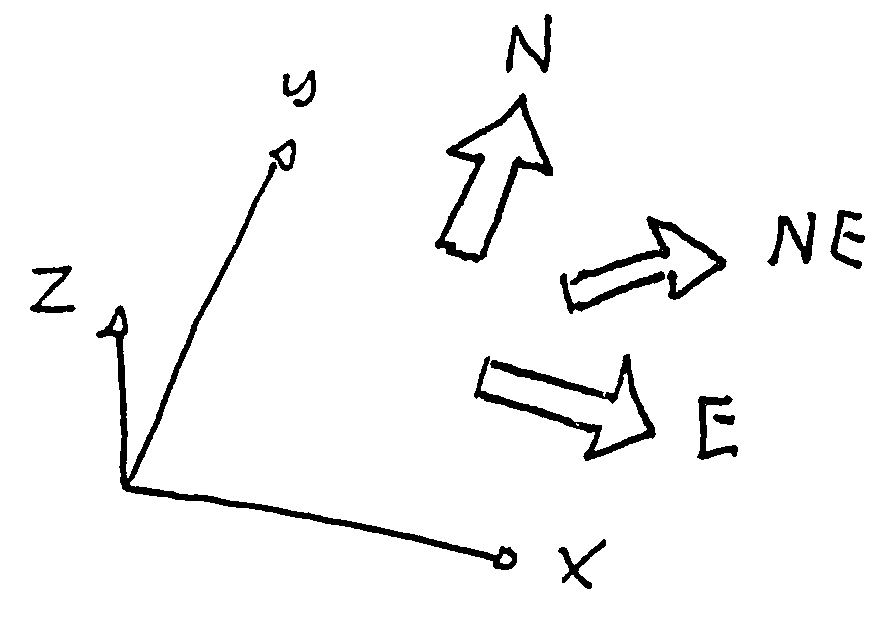
\includegraphics[height=3.5cm]{2021-1-C3/20210813_direcoes.pdf}
$$

\newpage

{\bf Exercício 4 (cont.)}

\ssk

d) Desenhe a trajetória associada a $α=0$, $β=-1$

e diga o nome da direção dela.

\ssk

e) Desenhe a trajetória associada a $α=-1$, $β=1$.

e diga o nome da direção dela.

\ssk

f) Quais são os valores mais simples de $α$ e $β$ ---

onde ``simples'' quer dizer ``$0$, $1$ ou $-1$'' --- que fazem

a trajetória ir pro nordeste? E pro sudoeste?

\bsk
\bsk

Nos próximos exercícios eu vou me referir a essas

trajetórias em que $α$ e $β$ são números ``simples''

pelos \ColorRed{nomes das direções} delas.


\newpage

% «zt-e-ztt-intro»  (to ".zt-e-ztt-intro")
% (c3m211qp 13 "zt-e-ztt-intro")
% (c3m211qa    "zt-e-ztt-intro")

{\bf O significado geométrico de $z_t$}

Nós sabemos calcular $z$, $z_t$ e $z_{tt}$ a partir de $t$,

e sabemos calcular $z$, $z_t$ e $z_{tt}$ em $t_0$.

\ssk

Com um pouquinho de esforço você deve ser

capaz de visualizar o que acontece perto de $t_0$...

o valor da primeira derivada, $(z_t)(t_0)$, diz o seguinte:

\def\LR{$\Longleftrightarrow$}

\msk

\begin{tabular}{lll}
$z$ aumenta quando $t$ aumenta (``crescente'')   &\LR& $(z_t)(t_0)>0$ \\
$z$ ``fica horizontal'' quando $t$ aumenta       &\LR& $(z_t)(t_0)=0$ \\
$z$ diminui quando $t$ aumenta (``decrescente'') &\LR& $(z_t)(t_0)<0$ \\
\end{tabular}

\bsk
\bsk

\ColorRed{

Veja o vídeo!!!

}

\ssk

{\footnotesize

\url{http://angg.twu.net/eev-videos/2021-1-C3-funcoes-quadraticas-3.mp4}

\url{https://www.youtube.com/watch?v=VwowES6EM3Y}

}

\newpage

{\bf O significado geométrico de $z_{tt}$}

Nos casos em que $z$ ``fica horizontal'' nós vamos usar

a segunda derivada, $(z_{tt})(t_0)$, pra ver se o gráfico de

$z(t)$ ``parece uma parábola'' ao redor de $t_0$, e se essa

parábola tem concavidade pra cima ou pra baixo:

\msk

\begin{tabular}{lll}
concavidade pra cima  &\LR& $(z_{tt})(t_0)>0$ \\
``parece horizontal'' &\LR& $(z_{tt})(t_0)=0$ \\
concavidade pra baixo &\LR& $(z_{tt})(t_0)<0$ \\
\end{tabular}

\bsk

Eu usei muitos termos informais de propósito.

No \ColorRed{próximo exercício} você vai tentar descobrir

\ColorRed{sem fazer contas} qual é o comportamento da $z$

em torno de $t_0$, e no \ColorRed{outro exercício} você vai

\ColorRed{fazer as contas} e vai ver se o seu olhômetro

funcionou direito.


\newpage

% «exercicio-5»  (to ".exercicio-5")
% (c3m211qp 15 "exercicio-5")
% (c3m211qa    "exercicio-5")

{\bf Exercício 5.}

\unitlength=20pt


Em cada um dos desenhos dos próximos slides diga

o que acontece quando a trajetória $(x(t),y(t))$ anda

em uma das oito direções simples, que são:

\msk

norte, nordeste, leste, sudeste,

sul, sudoeste, oeste, noroeste.

\bsk

Use estas categorias na suas respostas:

\msk

$z$ cresce

$z$ decresce

$z$ faz uma parábola com concavidade pra cima

$z$ faz uma parábola com concavidade pra baixo

$z$ é ``muito horizontal''




%L qf = QuadraticFunction {x0=3, y0=2, a=2, Dx=0, Dy=0, Dxx=1, Dyy=1, Dxy=0}
%L srf = Surface.new(qf, 3, 2)
\pu
$$\QuadraticInPerspective{srf}
$$



\newpage

%L qf = QuadraticFunction {x0=3, y0=2, a=2, Dx=0, Dy=0, Dxx=1, Dyy=-1, Dxy=0}
%L srf = Surface.new(qf, 3, 2)
\pu
$$\QuadraticInPerspective{srf}
$$

\newpage

% «ztt-matematicos»  (to ".ztt-matematicos")
% (c3m211qp 18 "ztt-matematicos")
% (c3m211qa    "ztt-matematicos")
% (find-books "__analysis/__analysis.el" "thomas")
% (find-books "__analysis/__analysis.el" "thomas" "3 Differentiation")

{\bf Calculando $z_{tt}$ em ``notação de matemáticos''}

\ssk

Lembre que:

\msk

\begin{tabular}{rl}
1) & estamos usando $z=z(x,y)$, $x=x(t)$ e $y=y(t)$, \\
2) & matemáticos odeiam usar os mesmos nomes pra \\
   & variáveis e pra funções, \\
3) & pra traduzir $z=z(x,y)$, $x=x(t)$ e $y=y(t)$ pra \\
   & notação de matemáticos vamos ter que \ColorRed{escolher} nomes \\
   & pra ``função $x$'', pra ``função $y$'' e pra ``função $z$'', \\
   % &  \\
4) & $z(x,y)$ é uma função de dois argumentos e \\
   & $z(t) = z(x(t),y(t))$ é uma \ColorRed{outra} função, de um \\
   & argumento só, \\
5) & se você quer ser entendido faça as suas definições \\
   & explicitamente, se possível usando ``seja''s e \\
   & ``digamos que''s... \\
\end{tabular}

\newpage

% «ztt-matematicos-2»  (to ".ztt-matematicos-2")
% (c3m211qp 19 "ztt-matematicos-2")
% (c3m211qa    "ztt-matematicos-2")

{\bf Calculando $z_{tt}$ em ``notação de matemáticos'' (2)}

\ssk

\ColorRed{Digamos que:}
%
$$\begin{array}{rcl}
  x(t) &=& f(t), \\
  y(t) &=& g(t), \\
  z(x,y) &=& H(x,t), \\
  z(x(t),y(t)) &=& m(t) \\
  \end{array}
$$

\def\ddt{\frac{d}{dt}}
\def\ddx{\frac{d}{dx}}
\def\ddy{\frac{d}{dy}}
\def\ddz{\frac{d}{dz}}
\def\ppt{\frac{∂}{∂t}}
\def\ppx{\frac{∂}{∂x}}
\def\ppy{\frac{∂}{∂y}}
\def\ppz{\frac{∂}{∂z}}

Então
%
$$\begin{array}{rcll}
  z_t &=& \ddt z(t)         & \ColorRed{\text{(?!?!)}} \\
      &=& \ddt m(t) \\
      &=& \ddt z(x(t),y(t)) \\
      &=& \ddt H(f(t),g(t)) \\
      &=& \ppx H(f(t),g(t)) \ddt f(t) + \ppy H(f(t),g(t)) \ddt g(t) \\
      &=& H_x(f(t),g(t)) f'(t) + H_y(f(t),g(t)) g'(t) \\
  \end{array}
$$


\newpage

% «ztt-matematicos-3»  (to ".ztt-matematicos-3")
% (c3m211qp 20 "ztt-matematicos-3")
% (c3m211qa    "ztt-matematicos-3")

{\bf Calculando $z_{tt}$ em ``notação de matemáticos'' (3)}

\ssk

Continuando...
%
$$\begin{array}{rcll}
  z_t &=& z_t(t)            & \ColorRed{\text{(?!?!)}} \\
      &=& \ddt z(t)         \\
      &=& \ddt m(t)         \\
      &=& \ddt z(x(t),y(t)) \\
      &=& \ddt H(f(t),g(t)) \\
      &=& \ppx H(f(t),g(t)) \ddt f(t) + \ppy H(f(t),g(t)) \ddt g(t) \\
      &=& \ppx z(x(t),y(t)) \ddt x(t) + \ppy z(x(t),y(t)) \ddt y(t) \\
      &=& z_x(x(t),y(t)) x_t(t) + z_y(x(t),y(t)) y_t(t) \\
      &=& z_x x_t + z_y y_t \\
  \end{array}
$$


\newpage

Os próximos slides são material de apoio pra este vídeo aqui:

\ssk

{\footnotesize

\url{http://angg.twu.net/eev-videos/2021-1-C3-funcoes-quadraticas-4.mp4}

\url{https://www.youtube.com/watch?v=d0fnURoPI9Q}

}


\newpage

% «gardner-1»  (to ".gardner-1")
% (c3m211qp 22 "gardner-1")
% (c3m211qa    "gardner-1")

{\bf Do prefácio do Martin Gardner...}

\ssk

(p.14): (...) Here the height of the mercury column relative to the
water's temperature is a one-to-one function of one variable. (...) In
modern set theory this way of defining a function can be extended
\ColorRed{to completely arbitrary sets} of \ColorRed{numbers} for a
function that is described not by an \ColorRed{equation} but by a
\ColorRed{set of rules}.

% (find-books "__analysis/__analysis.el" "thompson-gardner")
% (find-sthompsongpage (+ 9  15)   "interval")
% (find-sthompsongtext (+ 9  15)   "interval")
% (find-sthompsongpage (+ 9  15)   "did not use the modern")
% (find-sthompsongtext (+ 9  15)   "did not use the modern")

\msk

(p.14): For \ColorRed{most} of the functions encountered in calculus,
the domain consists of a single interval of real numbers.

\msk

(p.15): We call such a function ``continuous'' if its graph can be
drawn without lifting the pencil from the paper, and ``discontinuous''
otherwise. (The complete definition of continuity, which is also
applicable to functions with more complicated domains, is beyond the
scope of this book.)

\newpage

% «gardner-2»  (to ".gardner-2")
% (c3m211qp 23 "gardner-2")
% (c3m211qa    "gardner-2")

{\bf Do prefácio do Martin Gardner... (2)}

\ssk

(p.15): Note that if a vertical line from the $x$ axis intersects more
than one point on a curve, the curve cannot represent a function
because it maps an $x$ number to more than one $y$ number. Figure 5 is
a graph that clearly is not a function because vertical lines, such as
the one shown dotted, intersect the graph at three spots. (It should
be noted that Thompson did not use the modern definition of
``function.'' For example the graph shown in Figure 30 of Chapter XI
fails this vertical line test, but Thompson considers it a function.)

% (find-sthompsonpage (+ 11 106)   "Fig. 30")
% (find-sthompsontext (+ 11 106)   "Fig. 30")
\thompsonpage{117}

\bsk

$\hspace*{1cm}
 % (find-latexscan-links "C3" "20210816_thompson_fig_30")
 % (find-xpdf-page "~/LATEX/2021-1-C3/20210816_thompson_fig_30.pdf")
 \myvcenter{
 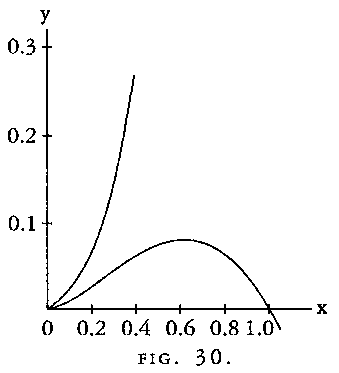
\includegraphics[height=2cm]{2021-1-C3/20210816_thompson_fig_30.pdf}
 }
 %
 \qquad
 \begin{array}[c]{rcl}
 (y-x^2)^2 &=& x^5 \\
 y-x^2 &=& \pm \; x^{5/2} \\
 y &=& x^2 \pm \, x^{5/2} \\
 \end{array}
$

\newpage


% «thompson-1»  (to ".thompson-1")
% (c3m211qp 24 "thompson-1")
% (c3m211qa    "thompson-1")

{\bf Do capítulo ``III. On Relative Growings'' do Thompson}

\ssk

Whenever we use differentials $dx$, $dy$, $dz$, etc., the existence of
some kind of relation between $x$, $y$, $z$, etc., is implied, and
this relation is called a ``function'' in $x$, $y$, $z$, etc.; the two
expressions given above, for instance, namely $\frac{y}{x} = \tan
30^{∘}$ and $x^2 + y^2 = ℓ^2$, are functions of $x$ and $y$. Such
expressions contain implicitly (that is, contain without distinctly
showing it) the means of expressing either $x$ in terms of $y$ or $y$
in terms of $x$, and for this reason they are called implicit
functions in $x$ and $y$; they can be respectively put into the forms...

\ssk

% (find-sthompsonpage (+ 11 13) "the existence of some kind of relation")
% (find-sthompsontext (+ 11 13) "the existence of some kind of relation")
\thompsonpage{24}

\newpage

% «thompson-2»  (to ".thompson-2")
% (c3m211qp 25 "thompson-2")
% (c3m211qa    "thompson-2")

{\bf Do capítulo ``III. On Relative Growings'' do Thompson}

\ssk

(...) We see that an explicit function in $x$, $y$, $z$, etc., is
simply something the value of which changes when $x$, $y$, $z$, etc.,
are changing, either one at the time or several together. Because of
this, the value of the explicit function is called the dependent
variable, as it depends on the value of the other variable quantities
in the function; these other variables are called the independent
variables because their value is not determined from the value assumed
by the function. For example, if $u = x^2 \sinθ$, $x$ and $θ$ are the
independent variables, and $u$ is the dependent variable.

\ssk

% (find-sthompsonpage (+ 11 14) "explicit function")
% (find-sthompsontext (+ 11 14) "explicit function")
% (find-sthompsonpage (+ 11 14) "dependent variable")
% (find-sthompsontext (+ 11 14) "dependent variable")
\thompsonpage{25}


\newpage

% «thompson-3»  (to ".thompson-3")
% (c3m211qp 26 "thompson-3")
% (c3m211qa    "thompson-3")

{\bf Do capítulo ``III. On Relative Growings'' do Thompson}

\ssk

Sometimes the exact relation between several quantities $x$, $y$, $z$
either is not known or it is not convenient to state it; it is only
known, or convenient to state, that there is some sort of relation
between these variables, so that one cannot alter either $x$ or $y$ or
$z$ singly without affecting the other quantities; the existence of a
function in $x$, $y$, $z$ is then indicated by the notation $F(x, y,
z)$ (implicit function) or by $x = F (y, z)$, $y = F (x, z)$ or $z = F
(x, y)$ (explicit function). Sometimes the letter $f$ or is used
instead of $F$, so that $y = F (x)$, $y = f (x)$ and $y = (x)$ all
mean the same thing, namely, that the value of $y$ depends on the
value of $x$ in some way which is not stated.

\ssk

% (find-sthompsonpage (+ 11 14) "z = F (x, y) (explicit function)")
% (find-sthompsontext (+ 11 14) "z = F (x, y) (explicit function)")
\thompsonpage{25}

\newpage

% «thompson-inversa-1»  (to ".thompson-inversa-1")
% (c3m211qp 27 "thompson-inversa-1")
% (c3m211qa    "thompson-inversa-1")

{\bf Do capítulo ``XIII. Other useful dodges'' do Thompson}

\ssk

It can be shown that for all functions which can be put into the
inverse form, one can always write
%
$$\frac{dy}{dx} · \frac{dx}{dy} = 1
  \qquad
  \text{or}
  \qquad
  \frac{dy}{dx} = \frac{1}{\frac{dx}{dy}}
  \; .
$$

% (find-sthompsonpage (+ 11 128)   "Differential of an Inverse Function")
% (find-sthompsontext (+ 11 128)   "Differential of an Inverse Function")
\thompsonpage{139}

\bsk
\bsk

You will surely realize from this chapter and the preceding, that in
many respects the calculus is an art rather than a science: an art only
to be acquired, as all other arts are, by practice. Hence you should
work many examples, and set yourself other examples, to see if you can
work them out, until the various artifices become familiar by use.


% (find-sthompsonpage (+ 11 130) "art rather than a science")
% (find-sthompsontext (+ 11 130) "art rather than a science")
\thompsonpage{141}

\newpage

% «thompson-inversa-2»  (to ".thompson-inversa-2")
% (c3m211qp 28 "thompson-inversa-2")
% (c3m211qa    "thompson-inversa-2")

{\bf Do capítulo ``XIII. Other useful dodges'' (2)}

\ssk

Um modo de traduzir esse ``$\frac{dy}{dx} · \frac{dx}{dy}$'' pra

``notação de matemáticos'' é supor que

$y(x) = f(x)$ e $x(y) = g(y)$, e que o

nosso ponto base é $(x,y) = (x,f(x))$...

\msk

(Também poderia ser $(x,y) = (g(y),y)$).

$$\begin{array}{rcl}
  \frac{dy}{dx}·\frac{dx}{dy} &=& \ddx y · \ddy x \\
                              &=& \ddx y(x) · \ddy x(y) \\
                              &=& \ddx f(x) · \ddy g(y) \\
                              &=& \ddx f(x) · \ddy g(y) \\
                              &=& f'(x) · g'(y) \\
                              &=& f'(x) · g'(y(x)) \\
                              &=& f'(x) · g'(f(x)) \\
  \end{array}
$$

\newpage

% «g-m-diff»  (to ".g-m-diff")
% (c3m211qp 29 "g-m-diff")
% (c3m211qa    "g-m-diff")

{\bf Do capítulo ``X. Geometrical Meaning of Differentiation''}

% (find-sthompsonpage (+ 11  75) "X. Geometrical Meaning of Differentiation")
% (find-sthompsontext (+ 11  75)    "GEOMETRICAL MEANING OF DIFFERENTIATION")

Se $y$ é uma função de $x$,

então $y_x = \frac{dy}{dx}$ também é uma função de $x$...

ou seja, $y_x = y_x(x)$.

% (find-sthompsonpage (+ 11 79) "Fig. 12")
% (find-sthompsontext (+ 11 79) "Fig. 12")
\thompsonpage{90}

$$
% (find-latexscan-links "C3" "20210817_thompson_fig_12")
% (find-xpdf-page "~/LATEX/2021-1-C3/20210817_thompson_fig_12.pdf")
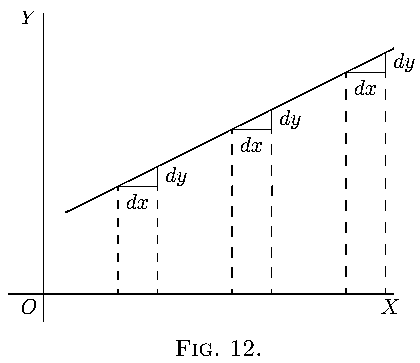
\includegraphics[height=4cm]{2021-1-C3/20210817_thompson_fig_12.pdf}
\qquad
% (find-latexscan-links "C3" "20210817_thompson_fig_13")
% (find-xpdf-page "~/LATEX/2021-1-C3/20210817_thompson_fig_13.pdf")
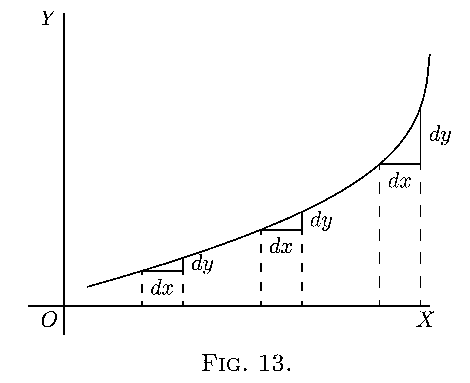
\includegraphics[height=4cm]{2021-1-C3/20210817_thompson_fig_13.pdf}
$$

% ...e temos $y_x=y_x(x)$. Podemos definir $w(x)=y_x(x)$



\newpage

% «useful-dodge»  (to ".useful-dodge")
% (c3m211qp 30 "useful-dodge")
% (c3m211qa    "useful-dodge")

{\bf ``A useful dodge''}

% ``IX. Introducing a Useful Dodge''

\ssk

O capítulo IX do Thompson ---

chamado ``IX. Introducing a Useful Dodge'' ---

é sobre um truque muito bom pra calcular derivadas

complicadas que faz muito mais sentido em ``notação

de físicos'' do que em ``notação de matemáticos'',

e que se baseia em \ColorRed{inventar variáveis novas}.

\msk

Link pro capítulo:

\ssk

{\footnotesize

% (find-sthompsonpage (+ 11  66) "IX. Introducing a Useful Dodge")
% (find-sthompsontext (+ 11  66)     "INTRODUCING A USEFUL DODGE")
% https://www.gutenberg.org/files/33283/33283-pdf.pdf#page=77
\url{https://www.gutenberg.org/files/33283/33283-pdf.pdf#page=77}

}


\newpage

% «exercicio-6»  (to ".exercicio-6")
% (c3m211qp 31 "exercicio-6")
% (c3m211qa    "exercicio-6")

{\bf Exercício 6.}

Refaça você mesmo os exemplos (1) até (7) desse capítulo

do Thompson pra ter certeza de que você entendeu o truque.

\msk

Link pro vídeo com dicas:

\ssk

{\footnotesize

\url{http://angg.twu.net/eev-videos/2021-1-C3-funcoes-quadraticas-5.mp4}

\url{https://www.youtube.com/watch?v=Ubc7wXK22fM}

}


\newpage

% «derivada-direcional»  (to ".derivada-direcional")
% (c3m211qp 32 "derivada-direcional")
% (c3m211qa    "derivada-direcional")

{\bf Derivada direcional (Bortolossi)}

% (find-bortolossi8page (+ -290 291) "8. Derivadas direcionais e o vetor gradiente")
% (find-bortolossi8page (+ -290 296)   "Definição 8.1. (Derivada direcional)")
% (find-bortolossi8page (+ -290 298) "8.2. O vetor gradiente")
% (find-bortolossi8page (+ -290 302)   "direção de maior crescimento")

O Bortolossi define a derivada direcional

deste jeito, na p.296 do capítulo 8 dele:

$$\frac{∂f}{∂𝐛v}(𝐛p) =
  \lim_{t→0} \frac{ f(𝐛p + t·𝐛v) - f(𝐛p) }{t}
$$

\msk

Digamos que $f:\R^2→\R$, que os argumentos da $f$

se chamem $x$ e $y$, que $𝐛p=(x_0,y_0)$, que o vetor $𝐛v$

seja $(α,β)$, e que $z=z(x,y)=f(x,y)$.

Então isto vira:
%
$$\begin{array}{rcl}
  \D \frac{∂z}{∂(α,β)}(x_0,y_0)
    &=& \D \lim_{ε→0} \frac{ z((x_0,y_0) + ε(α,β)) - z(x_0,y_0) }{ε} \\
    &=& \D \lim_{ε→0} \frac{ z(x_0+εα,y_0+εβ) - z(x_0,y_0) }{ε}
  \end{array}
$$

\newpage

{\bf Uma gambiarra...}

Digamos que $ε$ seja muito pequeno (``infinitesimal'').

O Bortolossi explica --- leia as páginas 291 a 294 dele! ---

que os casos mais básicos, que queremos generalizar,

são estes: $\frac{∂f}{∂(1,0)} = \frac{∂f}{∂x}$ e
%
$\frac{∂f}{∂(0,1)} = \frac{∂f}{∂y}$.

Então:
%
$$\begin{array}{rcl}
  z(x_0+εα,y_0+εβ) &≈& z(x_0,y_0)
                     + z_x(x_0,y_0)·εα
                     + z_y(x_0,y_0)·εβ \\
                   &=& z + z_x εα + z_y εβ \\
  \end{array}
$$

$$\begin{array}{rcl}
                       z(x_0+εα,y_0+εβ) - z(x_0,y_0)      &≈& z_x εα + z_y εβ \\[5pt]
             \D \frac{ z(x_0+εα,y_0+εβ) - z(x_0,y_0) }{ε} &≈& z_x α + z_y β \\[10pt]
  \lim_{ε→0} \D \frac{ z(x_0+εα,y_0+εβ) - z(x_0,y_0) }{ε} &=& z_x α + z_y β \\
  \end{array}
$$

\newpage

{\bf Uma gambiarra... (2)}

$$\begin{array}{rcl}
  \D \frac{∂z}{∂(α,β)}(x_0,y_0)
    &=& \D \lim_{ε→0} \frac{ z((x_0,y_0) + ε(α,β)) - z(x_0,y_0) }{ε} \\
    &=& \D \lim_{ε→0} \frac{ z(x_0+εα,y_0+εβ) - z(x_0,y_0) }{ε} \\[5pt]
    &=& z_x(x_0,y_0)·α + z_y(x_0,y_0)·β \\
  \D \frac{∂z}{∂(α,β)}
    &=& z_x·α + z_y·β \\
    &=& \pmat{z_x & z_y} · \pmat{α \\ β} \\
    &=& Dz · \pmat{α \\ β} \\
  \end{array}
$$




% (find-thomas11-1page (+  25  159) "3.2" "Differentiation rules")
% (find-thomas11-1page (+  26  171) "3.3" "The derivative as a rate of change")
% (find-thomas11-1page (+  28  183) "3.4" "Derivatives of trigonometric functions")
% (find-thomas11-1page (+  30  190) "3.5" "The chain rule and parametric equations")
% (find-thomas11-1page (+  30  198)      "differentiating with a parameter")

%\printbibliography

\GenericWarning{Success:}{Success!!!}  % Used by `M-x cv'

\end{document}

%  ____  _             _         
% |  _ \(_)_   ___   _(_)_______ 
% | | | | \ \ / / | | | |_  / _ \
% | |_| | |\ V /| |_| | |/ /  __/
% |____// | \_/  \__,_|_/___\___|
%     |__/                       
%
% «djvuize»  (to ".djvuize")
% (find-LATEXgrep "grep --color -nH --null -e djvuize 2020-1*.tex")

 (eepitch-shell)
 (eepitch-kill)
 (eepitch-shell)
# (find-fline "~/2021.2-C3/")
# (find-fline "~/LATEX/2021-2-C3/")
# (find-fline "~/bin/djvuize")

cd /tmp/
for i in *.jpg; do echo f $(basename $i .jpg); done

f () { rm -v $1.pdf;  textcleaner -f 50 -o  5 $1.jpg $1.png; djvuize $1.pdf; xpdf $1.pdf }
f () { rm -v $1.pdf;  textcleaner -f 50 -o 10 $1.jpg $1.png; djvuize $1.pdf; xpdf $1.pdf }
f () { rm -v $1.pdf;  textcleaner -f 50 -o 20 $1.jpg $1.png; djvuize $1.pdf; xpdf $1.pdf }

f () { rm -fv $1.png $1.pdf; djvuize $1.pdf }
f () { rm -fv $1.png $1.pdf; djvuize WHITEBOARDOPTS="-m 1.0 -f 15" $1.pdf; xpdf $1.pdf }
f () { rm -fv $1.png $1.pdf; djvuize WHITEBOARDOPTS="-m 1.0 -f 30" $1.pdf; xpdf $1.pdf }
f () { rm -fv $1.png $1.pdf; djvuize WHITEBOARDOPTS="-m 1.0 -f 45" $1.pdf; xpdf $1.pdf }
f () { rm -fv $1.png $1.pdf; djvuize WHITEBOARDOPTS="-m 0.5" $1.pdf; xpdf $1.pdf }
f () { rm -fv $1.png $1.pdf; djvuize WHITEBOARDOPTS="-m 0.25" $1.pdf; xpdf $1.pdf }
f () { cp -fv $1.png $1.pdf       ~/2021.2-C3/
       cp -fv        $1.pdf ~/LATEX/2021-2-C3/
       cat <<%%%
% (find-latexscan-links "C3" "$1")
%%%
}

f 20201213_area_em_funcao_de_theta
f 20201213_area_em_funcao_de_x
f 20201213_area_fatias_pizza



%  __  __       _        
% |  \/  | __ _| | _____ 
% | |\/| |/ _` | |/ / _ \
% | |  | | (_| |   <  __/
% |_|  |_|\__,_|_|\_\___|
%                        
% <make>

 (eepitch-shell)
 (eepitch-kill)
 (eepitch-shell)
# (find-LATEXfile "2019planar-has-1.mk")
make -f 2019.mk STEM=2021-2-C3-funcoes-quadraticas veryclean
make -f 2019.mk STEM=2021-2-C3-funcoes-quadraticas pdf

% Local Variables:
% coding: utf-8-unix
% ee-tla: "c3q"
% ee-tla: "c3m212q"
% End:
